\scanpage{96}
Nice , 11 Septembre 1967\\

Mon cher Grothendieck ,\\

Merci de ta lettre du 27/8 trouvée en arrivant ici , et du contre-exemple , qui ne m'étonne p\unsure{\deleted{q}a|\deleted{a}q}s . Mais je ne suis toujours pas convaincu que pour les Modules de présentation finie , sans condition noethérienne , la condition a) de (10.10.5) entraîne c) . \unsure{\deleted{X}C|\deleted{C}}ela irait tout seul si l'on savait que l'on a une suite exacte $\text{\uline{$O$}}_{\text{\uline{$X$}}}^{p}\handwritten{\to}\text{\uline{$O$}}_{\text{\uline{$X$}}}^{q}\handwritten{\to}\text{\uline{$F$}}\handwritten{\to}0$ , mais par définition cela \deleted{\unsure{ne}} n'est vrai que localement , et toute l'astuce de la démonstration actuelle consiste à se ramener à ce cas , en fabriquant un $\text{\uline{$G$}}=M^{\handwritten{\Delta}}$ et un homomorphisme canonique $\text{\uline{$F$}}\handwritten{\to}\text{\uline{$G$}}$ dont il ne reste plus qu'à prouver qu'il est bijectif , ce qui est une affaire locale

La construction de \uline{$G$} faite dans le texte actuel est on ne peut plus naturelle , mais utilise malheureusement l'implication b)$\handwritten{\Rightarrow}$a) qui est fausse dans le cadre de la présentation finie . Le canular me semble provenir de ce qu'on sait bien que $\text{\uline{$F$}}_n=\overset{\handwritten{\sim}}{M}_n$ , où $M_n$ est un $A_n$-module de présenta\unsure{\deleted{y}t|\deleted{t}y}ion finie , mais il faut ensuite passer à la limite projective \reversemarginpar\margin{\handwritten{\shortstack[l]{cf.\\EGA $\overline{\text{\uline{IV}}}$\\18.\unsure{3}.2.1.}}}\normalmarginpar et on retombe sur les canulars Artin-Rees ; si l'on avait des suites exactes $A_n^p\handwritten{\to}A_n^q\handwritten{\to}M_n\handwritten{\to}0$ avec $p$ et $q$ \uline{fixes} , on aurait gagné , mais comment les obtenir , je ne vois rien qui permette de limiter le nombre des générateurs ou des relations dans les $M_n$ . Bref , je suis tout aussi bloqué pour \deleted{\unsure{la|le}} a)$\handwritten{\Rightarrow}$c) que pour b)$\handwritten{\Rightarrow}$a) et j'ai des doutes sur la validité du théorème .

J'ai noté tes remarques sur l'Introduction , que je rédigerai lorsque j'aurai terminé le § 10 .

Bien entendu , je suis tout à fait d'accord pour prendre le papier de Serre ; donne-le à Mlle Rolland pour qu'elle l'envoie aux Presses , après avoir marqué la \uline{date de réception} du Ms. Même procédure \reversemarginpar\margin{\figure{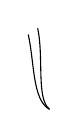
\begin{tikzpicture}[x=1cm,y=1cm]
\draw (0,0.95) .. controls (0.08,0.6) and (0.05,0.12) .. (0.27,0);
\draw (0.12,1.03) .. controls (0.2,0.65) and (0.1,0.14) .. (0.27,0);
\end{tikzpicture}}}\normalmarginpar pour les mém\unsure{\deleted{p}o|\deleted{o}p|p}ires de Segal quand tu les auras ; pense seulement à me dire combien cela fait de pages dactylographiées .

Meilleures amitiés\\
\handwritten{J A Dieudonné}\\
% archive sheet number: 95
